\documentclass[12pt]{article}
\usepackage[english]{babel}
\usepackage[utf8x]{inputenc}
\usepackage{amsmath}
\usepackage[hyphens]{url}
\usepackage{hyperref}
\usepackage{csquotes}
\usepackage{minted}
\usepackage{apacite}
\usepackage{graphicx}
\usepackage{fancyhdr}
\usepackage[colorinlistoftodos]{todonotes}
\setlength{\parindent}{0in}
\hypersetup{
    colorlinks=false,
    urlcolor=black
}

% Header
\pagestyle{fancy}
\fancyhead{}
\fancyhead[l]{G53SQM}
\fancyhead[R]{\hyperref[toc]{Table of Contents}}

\begin{document}
\begin{titlepage}

\newcommand{\HRule}{\rule{\linewidth}{0.5mm}}

\center 
\textsc{\LARGE University of Nottingham}\\[1.5cm]

\includegraphics[scale=0.4]{images/uon.jpg}\\[1cm]
\textsc{\Large Software Quality Assurance}\\[0.5cm]
\textsc{\large G53SQM}\\[0.5cm]

\HRule \\[0.4cm]
{ \huge \bfseries Final Report}\\[0.4cm]
\HRule \\[1.5cm]

\begin{minipage}{0.4\textwidth}
\begin{flushleft}
\emph{Authors:}\\
\vspace{0.1cm}
Rishi \textsc{Parmar}\\
Kieran \textsc{Sohal}\\
Annabel \textsc{Kenny}
\end{flushleft}
\end{minipage}
~
\begin{minipage}{0.4\textwidth}
\begin{flushright} 
\emph{Professor:} \\
Dr. Paul \textsc{Tennant}
\end{flushright}
\end{minipage}\\[2cm]

{\large \today}\\[2cm]

% 
\includegraphics[scale=0.4]{uon.png}\\[1cm]

\vfill

\end{titlepage}

\tableofcontents
\label{toc}
\addtocontents{toc}{~\hfill\textbf{Page}\par}

\newpage

\section{Report Summary}

In this module, we have created a simple 2D Java game called `Shoot The Block', a short demo for which can be found \underline{\href{https://media.giphy.com/media/woCCylWbiKvxFW0PJP/giphy.gif}{here}}. The objective of the game is to see how many `blocks' the user can shoot in the specified time period. The time period and block spawn rate can both be modified by changing the relevant constant in our dedicated Constants class. \\


Over the course of the project, we used various \emph{Quality Assurance} strategies as well as more general \emph{Agile} strategies where possible. Such strategies included usage of: 

\begin{itemize}
    \item Project Management Software
    \item Version Control Systems (VCS)
    \item Black-Box Testing
    \item White-Box Testing
    \item Code Reviews
    \item Code Conventions
    \item Code Metrics
    \item Sprint Planning
    \item Sprint Retrospectives
    \item One Formal Technical Review
\end{itemize}

 This report will present our experiences using all of the above; going into detail as to how we implemented these strategies and evaluating their effectiveness having done so.
 
 \newpage
 
 \section{Software Quality Assurance Plan}
 
 \subsection{Scope and Aim}
 The main purpose of this plan is to outline the various software tools and processes that will be used in the project. This document should be constantly referred to in order to ensure that the processes defined are followed correctly. Doing so is important as it will ensure that the final product is one of high quality, with minimal defects present. 
 
 \subsection{That which is being QA'd}
 The game is a simple one, and we will aim to avoid using any external game libraries as this is a surefire way to decrease overall test coverage. By using only our own code, we will be in a position where we have a better overall understanding of the codebase. Consequently, we will be able to test more of the codebase which is why overall coverage will be greater.
 
 \subsection{Roles, Responsibilities \& Methodologies}
 A traditional Agile software team consists of: a Project Manager, Developer(s), Tester(s), Business Analyst(s). Despite being a group of three, we are keen to have all roles fulfilled. Naturally, members will be required to fulfil more than one role:
 
 \begin{itemize}
     \item Rishi $\longrightarrow$ Project Manager (PM) \& Developer
     \item Kieran $\longrightarrow$ Tester (QA) \& Code Reviewer
     \item Annabel $\longrightarrow$ Business Analyst (BA) \& Metrics collector
 \end{itemize}
 
The PM is responsible for making sure that the team sticks to the processes and tools mentioned in this plan. The PM also has the responsibility of making sure that every team member has work to do and are aware of what this work consists of. The developer is responsible for writing the game code and unit tests for said code. \\
 
The BA defines the requirements for the game and plays a role in ensuring that such requirements are met. The BA has to consider and represent the user's best interests. Metrics collection involves using an IDE plugin to obtain various code metrics such as `number of lines of code'. This data must then be collected, formatted and presented in a way that provides useful insights for future development. \\
 
The QA manually tests the game, using the requirements as a baseline for determining whether or not the product quality is satisfactory. The QA should also define test plans and is free to undertake `exploratory testing.' This involves trying different things out that may not be on the requirements --- the purpose of which is to find any defects that may otherwise be missed. \\

Agile's most natural form involves two-week sprint cycles with more than one story (chunk of work) for each sprint. Sticking to a two or even a one week cycle at University is unlikely to be successful. This is due to the nature of University work; one week a student may be busy with deadlines, another week they may be free. It is clear that --- for the purpose of this project --- agile can't be adopted in its most well-known form. The solution to this problem is not to ditch the methodology altogether, but to adapt it to our needs. Instead of working in timed sprints, we will base our work around the stories. The total work will probably amount to three or four stories. Each story will be treated like it is an Agile-like Sprint in the respect that there will be a BA/QA/DEV at the beginning, and a retrospective at the end. More information about the project-level processes and tools used will be outlined in the later in this plan.

\newpage

 \subsection{The Processes and their Purposes}
 \vspace{0.3cm}
\noindent\makebox[\textwidth]{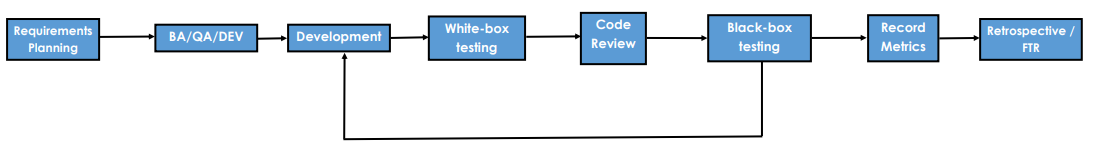
\includegraphics[width=\paperwidth]{images/processes.png}}

The above flow represents a whole Sprint, or Story. 

\begin{enumerate}
    \item \textbf{Requirements planning} is done by the BA. It involves creating user stories aimed at making it clear to the developer what would constitute a \emph{quality} end-product. Requirements will be written for each sprint. The requirements from Sprint 1 may or may not still be relevant in Sprint 2 or 3. The ability to change requirements is one of the advantages of using an Agile-influenced approach.
    \item \textbf{BA/QA/DEV} is a meeting format used by some Agile teams (it is also known as a `Three Amigos' meeting). In our case, this meeting will involve all three team members. The purpose of the meeting is to make sure everyone is on the same page regarding what is expected for the Sprint. A topic of conversation might be the \emph{requirements} --- making sure that everyone understands them or considering whether or not they ought to be changed. This meeting provides a apt opportunity to create the Development tasks and Test plans for the subsequent Sprint.
    \item \textbf{Development} is simply the programming segment of the Sprint. The development tasks should be broken down for each story so that no task has an estimate of more than a day. There will likely be three to four development tasks for each Sprint.
    \item \textbf{White-box testing} is a style of testing where the internal structure of the application is known to the tester. In our case, this will most likely take the form of unit tests which is why this occurs before code reviews and after development. 
    \item \textbf{Code reviews} are a way to ensure that code is good quality. Code might be bad quality if the coding conventions being used are not followed, or if the Developer simply makes any careless mistakes in their code. It is important to have a second-pair of eyes look at the code to spot any bad practices or errors.
    \item \textbf{Black-box testing} is a style of testing where the tester doesn't know the internal details of the application. In our case, this will take the form of \emph{acceptance testing} and \emph{exploratory testing}. Note how this particular task has a connection with the earlier `Development' task. This specific flow will occur if a defect is found during testing. In this scenario, the QA will have to raise the defect and the Developer will have to fix it.
    \item \textbf{Metrics recording} will be done towards the end of the Sprint. The data will be reviewed in the retrospective/FTR at the end of the Sprint. 
    \item \textbf{Retrospective/FTR} will occur at the end of the Sprint. There will only be one Formal Technical Review (FTR) which will be documented. The rest of the Sprints will follow a standard \emph{Retrospective} template. Namely, each group member will have to answer three questions: 
    \begin{itemize}
    \item What went well? 
    \item What didn't go so well? 
    \item What can we do to do better next time? 
    \end{itemize}
    The purpose of the retrospective is to provide a suitable avenue for group members to provide feedback which can be used to progress going forward.
\end{enumerate}

\newpage
 
\subsection{Tools, Methods, \& Storage}
 We will use Trello as our main project-management software. Trello will contain all of the tasks and there should be coloured labels that make it clear which team member each task is intended for. Trello is an intuitive tool that all group members have experience with. Trello can be used to store resource, such as the process flow diagram given above. The metrics will be recorded using an IDE but stored in a spreadsheet - preferably Google Sheets for optimal accessibility. This spreadsheet can be linked to Trello so that all relevant resources can be in one place. As for our Version Control System (VCS), we will use GitHub - mainly due to its familiarity.
 
\subsection{Standards and Practices}
\label{practices}
We will try to adhere to the \underline{\href{https://google.github.io/styleguide/javaguide.html}{Google Java Style Guide}}. This coding convention lays out several good and bad practices including those which relate to: constants usage, class naming, variable namingm and brace usage. The style guide also offers some advice on formatting \emph{JavaDocs}. We will aim to have JavaDocs on every method --- regardless of complexity --- as doing so can greatly enhance readability.
\section{Project Management Tool Usage}

We used Trello for much of our information storage and communication. We liked the idea of having one web-page which would act as a central hub for the project. The following page contains a screenshot of our Trello board, post project. Notice how the layout of each story closely mirrors the project process-flow diagram included earlier in this report.

% \includegraphics[scale=0.6]{trello1.png}
\noindent\makebox[\textwidth]{\includegraphics[scale=0.7]{images/trello1.png}}

The tickets were colour-coded in a way as to make it obvious who the task was intended for. Here is the colour key for these labels:

\begin{center}
    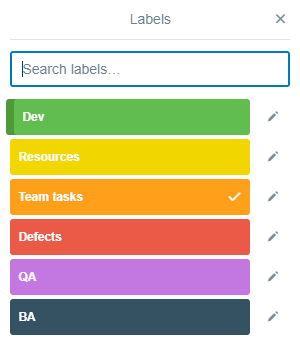
\includegraphics{images/trello2.png}
\end{center}

\section{Requirements}

As mentioned in the SQA plan, most of the requirements were Sprint-specific and defined at the beginning of the Sprint. The main reason for this is to allow for the change of requirements if necessary. There were, however some generic requirements which were always unlikely to change:

\subsection{Functional Requirements}

\begin{itemize}
    \item The box should disappear when it is clicked on.
    \item The application must count the number of boxes that have been clicked.
    \item The application should have a final screen which shows the score.
    \item The application should keep track of the time remaining.
\end{itemize}

\subsection{Non-Functional Requirements}

\begin{itemize}
    \item The game should be able to run on any computer-based operating system i.e. Windows, Linux, MacOS.
    \item Any text on the game screen should be large enough as to be easily readable.
    \item The codebase should be open-source --- perhaps with an MIT license.
    \item There should be no or minimal delay between user input and game response i.e. a mouseclick.
\end{itemize}

In addition to these generic requirements, we also included more specific story-level requirements. These were stored in the description of the `Requirements' task in Trello.

\subsection{Story 1}

    \begin{center}
        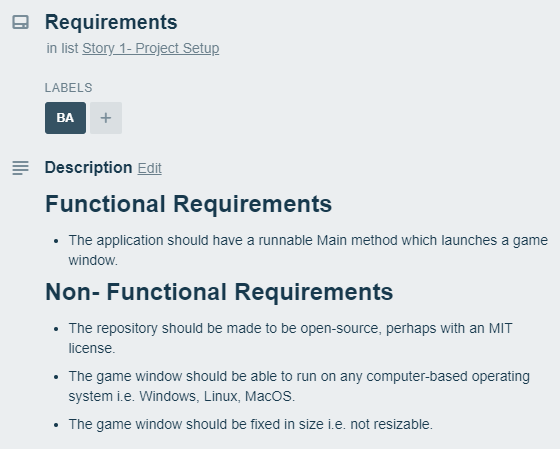
\includegraphics[scale=0.9]{images/story1}
    \end{center}

\subsection{Story 2}

    \begin{center}
        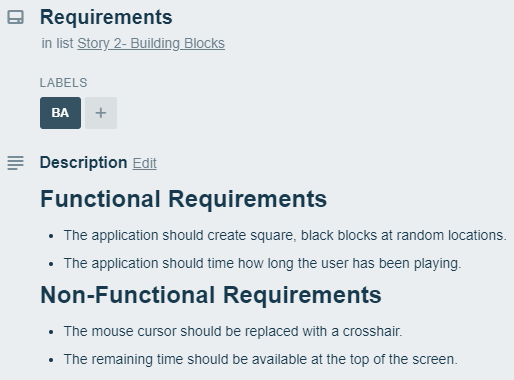
\includegraphics[scale=0.8]{images/story2}
    \end{center}

\subsection{Story 3}

    \begin{center}
        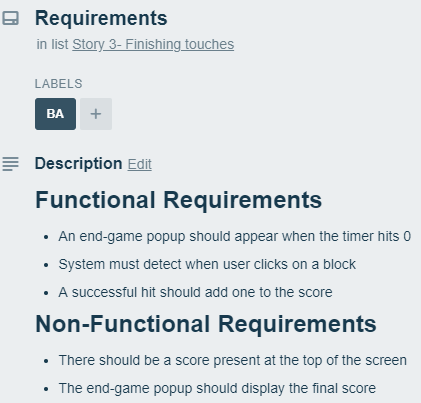
\includegraphics[scale=0.8]{images/story3}
    \end{center}
    
    
\section{Product Structure}
The overall product is probably too small to warrant creating a software architecture diagram. This is not to say that there is no architecture present. A good understanding of the overall design can be obtained by observing the file structure in a tree format:

\begin{minted}{bash}
|   pom.xml
|   README.md
|
|---src
    |---main
    |   |---java
    |           Block.java
    |           BlockHandler.java
    |           Constants.java
    |           Game.java
    |           HUD.java
    |           MouseClickListener.java
    |           Window.java
    |
    |---test
        |---java
                BlockHandlerTest.java
                BlockTest.java
                HudTest.java
                WindowTest.java
\end{minted}

The pom.xml is a Maven build file. Maven is similar to Gradle - it is a build system. This project uses a build system for a testing library called Mockito, which will be elaborated on later in this report. The rest of the project is simply split into \emph{main} (Java files that constitute the actual game) and \emph{test} (test files). 

\newpage

\section{Metrics}

Our metrics were updated on a continual basis. Most of the metrics we created were project-level i.e. they looked at all files in the project as a whole rather than individual files. Metrics were recorded towards the end of the Sprint, but before the Retrospective to allow us to discuss the data.

\subsection{Project-level Metrics}

\vspace{0.3cm}
\begin{center}
    \noindent\makebox[\textwidth]{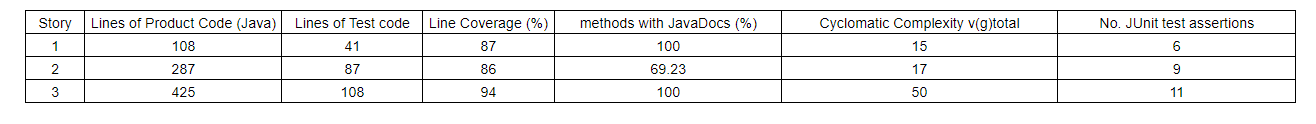
\includegraphics[width=\paperwidth]{images/Project_level.png}}
\end{center}

\begin{itemize}
    \item Lines of Product Code $\longrightarrow$ The number of lines of Java game code. This figure does not any code from the test classes or build scripts. We included this because it provides a rough estimate for how large a story is - at least in terms of features.
    \item Lines of Test code $\longrightarrow$ The number of lines of JUnit code. We included this statistic to gauge how much effort is being spent on unit testing throughout the project.
    \item Line Coverage $\longrightarrow$ The percentage of lines that are executed during a complete run of the game. If the value is low, it suggests that there are a lot of methods that exist in the application which aren't being executed - and therefore should be omitted. 
    \item Methods with JavaDocs $\longrightarrow$ We comitted to include JavaDocs on every method in our \underline{\hyperref[practices]{plan}}. This metric exists to alert us if this commitment is ever avoided.
    \item Cyclomatic Complexity v(g)total $\longrightarrow$ used to show the total number of paths that are available on a program. The more paths there are, the higher the complexity.
    \item No. JUnit assertions $\longrightarrow$ This metric actually shows the number of test \emph{methods} with assertions rather than simply the number of assertions. This is another metric that allows us to observe overall test coverage.
\end{itemize}
\newpage

Using this data, we were able to create several different charts that would update themselves over time. The metrics we decided to create charts for were: Line Coverage, JavaDoc Coverage, Complexity and JUnit Assertions.

\vspace{0.3cm}

\begin{center}
    \noindent\makebox[\textwidth]{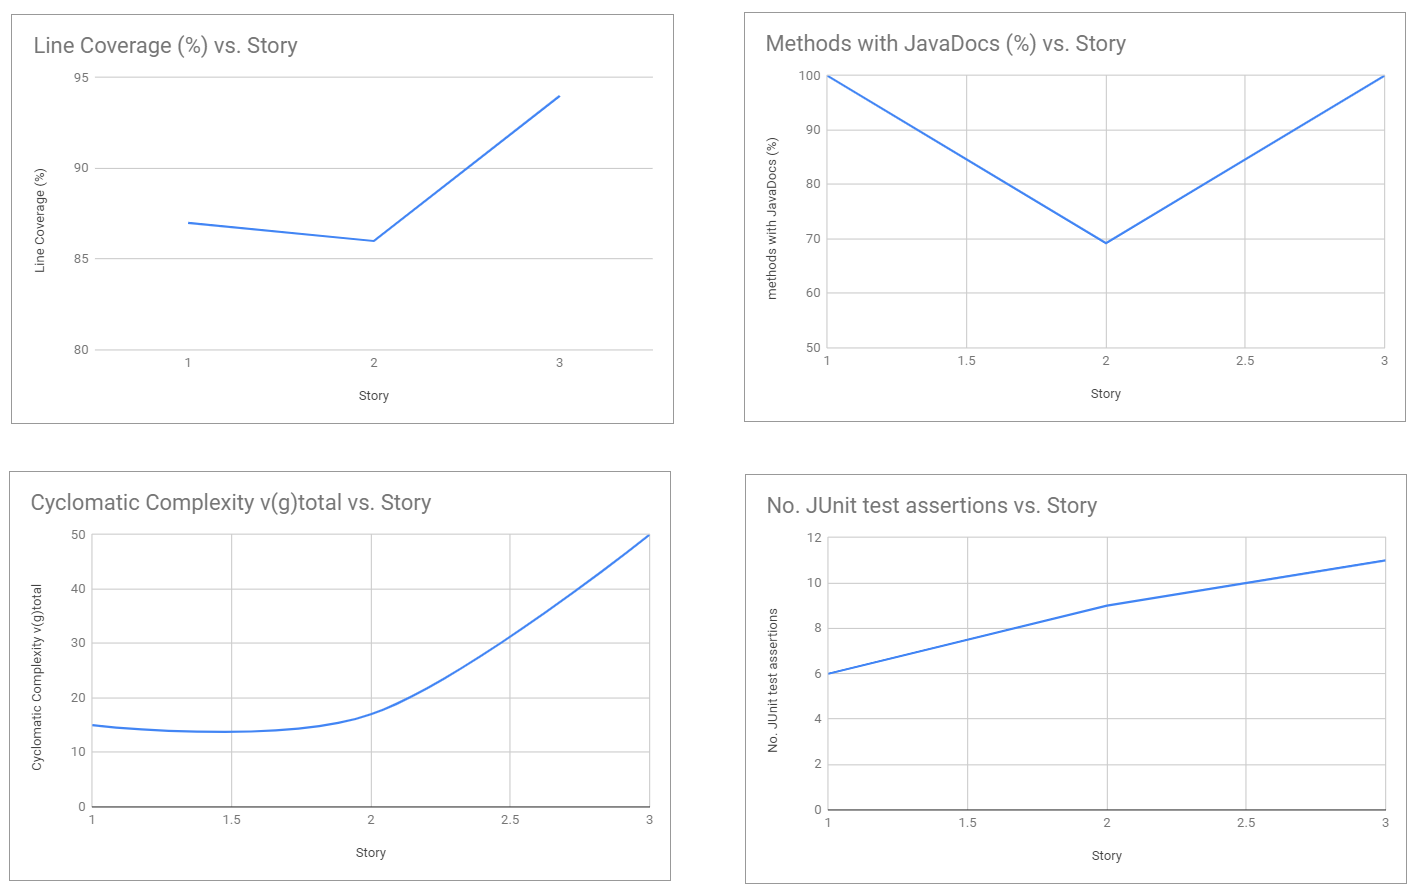
\includegraphics[width=\paperwidth]{images/charts.png}}
\end{center}

\newpage

The second Sprint was by far the most important Sprint to observe metrics purely because there were only three Sprints altogether. This is one of the reasons why we decided to hold the Formal Technical Review at the end of the second Sprint. The metrics charts above varied in their usefulness --- two of these charts prompted us to make a change/improvement while the other two were discussed but not acted upon.

\begin{itemize}
    \item Tracking line coverage allowed us to find a couple of methods that were not ever being called. We saw that at the end of the second Sprint the coverage wasn't only far from 100\%, but had also decreased. It was clear that there was a fair chunk of code that wasn't being run. Luckily for us, Intellij's `Run with Coverage' option shows the methods that did and did not run. Using this data, we were able to remove the unused methods which drastically improved overall coverage for Sprint 3. We are pleased with the 94\% coverage we managed to achieve. It is worth noting that 100\% coverage isn't necessarily desirable as some code is only meant to be run when something goes wrong. In this respect, line coverage as a metric can be slightly misleading.
    \item Tracking the percentage of methods with JavaDocs allowed us to observe a sharp reduction in JavaDoc coverage in Sprint 2. This was flagged in the FTR and was an easy problem to fix. 
    \item v(g)total is a metric that we concluded to be less than useful. This is because there is a natural correlation between the number of lines of code and the v(g)total. Both of these metrics can be misleading since each Story is bound to be different in terms of how much work/coding is required. We found that the tasks for Stories two and three were more complex than the first. It would have been more useful to record the complexity on a method-level rather than a project-level. This would allow us to see methods that are getting too complex and the action would be to break the method down. 
    \item The JUnit assertion chart showed that we did increase our coverage over time, but once again there were a couple of drawbacks of this method. The first drawback has already been mentioned - the metric counts the number of methods with assertions rather than simply the number of assertions. We had test methods which had more than one assertion which reduces the overall accuracy of the chart. It could be argued that an appropriate action would be to only have one assert per method; however, this would entail adapting our code based on the specific workings of one metric which is undesirable overall.
\end{itemize}

\subsection{Class-level Metrics}
Project-level metrics provide useful insight for the quality of the codebase as a whole, but they can often fail to identify smaller, lower-level problems. Considering this, we decided to include one class-level metric, namely the \emph{test coverage} for each class. 

\begin{center}
    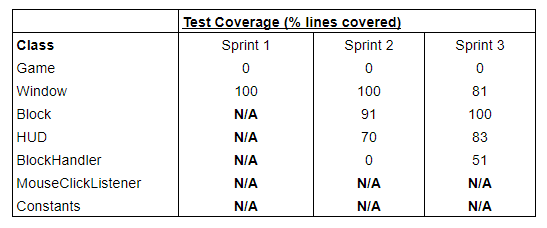
\includegraphics[scale=0.7]{images/class_level.png}
\end{center}

Forgetting to write Unit tests for a new class is a fairly easy mistake to make. This mistake was made following the creation of BlockHandler.java in Sprint 2. This metric makes it easy to see \emph{where} there is a lack of test coverage, which proved to be useful. It may be the case that we never realised the missing test file had we only used project-level metrics. It is worth noting, however, that 100\% test coverage isn't always desirable nor achievable. Some methods can be extremely difficult to Unit test. Other methods --- such as `getters and setters' --- are arguably not worth testing in the first place.

\section{Review Process}

Reviews occurred at the end of each Sprint and either took the form of a \emph{Retrospective} or in one case a \emph{Formal Technical Review}. FTR's offer an opportunity to evaluate whether or not the product quality sits at an acceptable level, and to discuss strategies for getting to that level if any aspects of the product are unsatisfactory. Retrospectives are less about the product and more about team dynamic.

\subsection{Retrospectives}

In the retrospective each group member had to answer three questions:

\begin{itemize}
\item What went well?
\item What didn’t go so well?
\item What can we do to do better next time?
\end{itemize}

One takeaway from the first Retrospective was that the team liked the format of the Trello board and deemed it to be intuitive. Members found it easy to know what they needed to do and liked how the Metrics spreadsheet link was available on the Trello page. Thus, it was decided that we would continue to use coloured labels for our tasks. \\

The second takeaway was that we perhaps didn't include enough development work for the first story. The state of the game at the end of Sprint one was a simple game window, which doesn't leave much to QA. Despite the lack of work to QA, we still had to follow the same processes which made us feel that we weren't very efficient with our time. Looking back at the Metrics, it is evident that while we made did well at following our processes, there wasn't code overall. As a result, we concluded that for the next Story/Sprint we would include more work which would result in less context-switching and greater efficiency.

\subsubsection{Formal Technical Review}

The FTR was different in several ways. For one, the FTR involved a `show and tell' which involved showing the game to two reviewers who were tasked with assessing the quality of the game thus far. To do this, the reviewers referred to all of the existing requirements on hand, checking them off one by one if they were judged to be acceptable. \\

During this meeting, one reviewer noticed that occasionally blocks could spawn on top of each other due to the random nature of their positioning. This meant that in some situations the user could destroy both blocks with one click, scoring two points in the process. It was never considered whether or not this game mechanic should exist and if so should exist as a non-functional requirement. We decided that we liked the mechanic and that it should be considered a \emph{feature} rather than a \emph{bug}. \\

We used this meeting as an opportunity to discuss the results of our metrics thus far. We found that we weren't hitting our goal of having JavaDocs on every method and that we had some methods that weren't doing anything at all. Thus, we found ourselves in a situation where all of the requirements were met, but the product lacked certain quality assurances. The reviewers were therefore unsure as to whether the product should be accepted completely or \emph{provisionally}. We decided to err on the side of caution and accept the product provisionally, citing the problems indicated by the metrics as those that needed to be solved.

\subsubsection{Code Reviews}

One of the advantages of pair programming is the ability to have two sets of eyes look at a piece of code. It is often the case that one developer will spot an error that the other is blind to, and vice-versa. The idea behind code reviews is similar, it is an opportunity to assess the quality of production code on a low level. GitHub provides a useful `comment' feature that makes this process very straight forward. 



\end{document}
